
\part{The equations and the algorithms}
\noindent \begin{flushright}
\textit{Paradoxically, it has turned out that game theory}\\
\textit{ is more readily applied to biology than }\\
\textit{to the field of economic behaviour for which }\\
\textit{it was originally designed.}\\
\textit{ }John Maynard Smith 
\par\end{flushright}

As anticipated, after an introduction to the classical game theory
and the evolutionary game theory, this chapter aims to study two partial
differential equations (PDEs) and to solve them numerically. Numerical
methods for PDE is a chaotic world. To move in it, we have first to
determine what type of PDE we want to solve, and then work on the
order of accuracy desired. Thus, considering a generic PDE of the
form:
\[
A\frac{\partial^{2}u}{\partial x^{2}}+B\frac{\partial^{2}u}{\partial x\partial y}+C\frac{\partial^{2}u}{\partial y^{2}}+D\frac{\partial u}{\partial x}+E\frac{\partial u}{\partial y}+F=0
\]

\begin{itemize}
\item If $B^{2}-AC<0$, the PDE is elliptic;
\item If $B^{2}-AC=0$, the PDE is parabolic;
\item If $B^{2}-AC>0$, the PDE is hyperbolic.
\end{itemize}
Below, after an analysis of the equations, we define, verify and validate
numerical methods for the investigated PDEs, and finally solve them
numerically.

\section{Classical game theory}

Game theory is the study of mathematical models of conflict and cooperation
between intelligent rational decision-makers. It provides general
mathematical techniques for analyzing situations in which two or more
individuals make decisions that will influence one another's welfare
\cite{myerson1991game}.
\begin{defn}
A strategic form game is any triplet $\Gamma$ of the form:
\[
\Gamma=\left\{ N,\left(C_{\ell}\right)_{\ell\in\mathcal{N}},\left(u_{\ell}\right)_{\ell\in\mathcal{N}}\right\} ,
\]
 where:
\end{defn}

\begin{enumerate}
\item $\mathcal{N}$ is the nonempty set of \textit{simultaneous-playing
rational players} in the game;
\item $C_{\ell}$ is the nonempty set of strategies (or \textit{pure strategies})
available to player $\ell$. In a strategic-form game $\Gamma$ each
player $\ell$ must choose one of the strategies $c_{\ell}$ in the
set $C_{\ell}$. We let $C$ denote the set of all possible strategy
profiles, i.e. \[C=\underset{\ell\in\mathcal{N}}{\textifsym{\BigCross}} C_{\ell}\]
so a pure strategy profile is:
\[
\mathbf{c}\coloneqq\left(c_{\ell}:\ell\in\mathcal{N}\right)
\]
\item $u_{\ell}$ is the payoff function from $C$ into the set of real
numbers $\mathbb{R}$, i.e.:
\begin{align*}
u_{\ell}: & C\rightarrow\mathbb{R}\\
 & \mathbf{c}\mapsto u_{\ell}\left(\mathbf{c}\right)
\end{align*}
It represents the expected payoff that player $\ell$ would get in
this game if $\mathbf{c}$ were the combination of strategies implemented
by the players. 
\end{enumerate}
The games that involve only two players can be represented with a
more convenient form: the \textit{payoff matrix}. The player labeled
with $1$ is called \textit{row player} and the player labeled with
$2$ is called \textit{column player}. The rows of the payoff matrix
are the pure strategies of the row player, $C_{1}=\left(R_{1},\dots,R_{m}\right)$,
while the columns are the pure strategies of the column player, $C_{2}=\left(T_{1},\dots,T_{n}\right)$.
The element on the $i^{th}$ row and on the $j^{th}$column has a
pair of values that represents the pair of the payoffs related to
the strategy profile $\left(R_{i},T_{j}\right)$. For example, in
the prisoner's dilemma both the prisoners have $C_{1}=C_{2}=\left\{ cooperate,\quad defect\right\} $
\begin{center}
\begin{tabular}{|c|c|c|}
\hline 
 & cooperate & defect\tabularnewline
\hline 
\hline 
cooperate & R,R & S,T\tabularnewline
\hline 
defect & T,S & P,P\tabularnewline
\hline 
\end{tabular}
\par\end{center}

The concept of pure strategy can be extended, assuming that the players
can play their pure strategies with certain probabilities.
\begin{defn}
Let $\Delta\left(C_{\ell}\right)$ be the set of the probability measure,
i.e.:
\[
\Delta\left(C_{\ell}\right)=\left\{ \bm{\sigma}_{\ell}=\left(p_{1},\dots,p_{k}\right)\in\mathbb{R}^{k}:p_{\ell}\geq0,\ \sum_{\ell=1}^{k}p_{\ell}=1\right\} 
\]
A mixed strategy for player $\ell$ is any $\bm{\sigma}_{\ell}\in\Delta\left(C_{\ell}\right)$
that specifies a probability $\bm{\sigma}_{\ell}\left(c_{\ell}\right)$
for every $c_{\ell}$ that player $\ell$ could play. In other terms
$\bm{\sigma}_{\ell}$ is a $\left(k-1\right)-simplex$. So a mixed
strategy profile is:

\[\bm{\sigma}\coloneqq\left(\bm{\sigma}_{\ell}:\ell\in\mathcal{N}\right)\in\underset{\ell\in\mathcal{N}}{\textifsym{\BigCross}} \Delta \left(C_{\ell}\right) \]For
2-players games we denote the mixed strategies by:
\begin{align*}
\mathbf{p} & \in\Delta\left(C_{1}\right)\\
\mathbf{q} & \in\Delta\left(C_{2}\right).
\end{align*}
The payoff function of the player $i$ in terms of the mixed strategies
become\begin{align}u_{\ell}:&\underset{\ell\in\mathcal{N}}{\textifsym{\BigCross}}\Delta\left(C_{\ell}\right)\rightarrow\mathbb{R}\\&\bm{\sigma}\mapsto u_{\ell}\left(\bm{\sigma}\right)\end{align}
and it can be computed by:
\[
u_{\ell}\left(\bm{\sigma}\right)=\sum_{c\in C}\prod_{j\in\mathcal{N}}\bm{\sigma}_{j}\left(c_{j}\right)u_{\ell}\left(\mathbf{c}\right)
\]
\end{defn}

\begin{rem}
For games with 2 players, the payoff matrix allows us to compute the
payoff with a simple matrix multiplication, i.e.:
\[
u_{\ell}\left(\mathbf{p},\mathbf{q}\right)=\mathbf{p}{}^{T}A\mathbf{q}
\]
For example, consider the row player of the prisoner's dilemma playing
the strategy $\mathbf{p}=\left(\begin{array}{c}
p_{C}\\
p_{D}
\end{array}\right)$ against the column player playing $\mathbf{q}=\left(\begin{array}{c}
q_{C}\\
q_{D}
\end{array}\right)$ and its payoff matrix is:
\[
A=\left(\begin{array}{cc}
R & S\\
T & P
\end{array}\right)
\]
So, the payoff is:
\[
u_{1}\left({\bf p},{\bf q}\right)=\left(\begin{array}{cc}
p_{C} & p_{D}\end{array}\right)\left(\begin{array}{cc}
R & S\\
T & P
\end{array}\right)\left(\begin{array}{c}
q_{C}\\
q_{D}
\end{array}\right)
\]
 Note, we write the pure strategies as a vector ${\bf e_{\ell}}$
with $1$ on the $\ell-th$ component and zero otherwise. For instance,
the cooperate strategy in the prisoner's dilemma is:
\[
{\bf e}_{C}=\left(\begin{array}{c}
1\\
0
\end{array}\right).
\]
\end{rem}

Now, we can introduce one of the most important concept of the game
theory: the \textit{Nash equilibrium. }
\begin{defn}
Given a strategic form game:
\[
\Gamma=\left\{ N,\left(C_{\ell}\right)_{\ell\in\mathcal{N}},\left(u_{\ell}\right)_{\ell\in\mathcal{N}}\right\} ,
\]
 a mixed strategy profile:

\[\bm{\sigma}\coloneqq\left\{\bm{\sigma}_{\ell}:\ell\in\mathcal{N}\right\} \in \underset{\ell\in\mathcal{N}}{\textifsym{\BigCross}}\Delta\left(C_{\ell}\right)\]is
a Nash equilibrium if:
\[
\forall\ell\in\mathcal{N},\quad u_{\ell}\left(\bm{\sigma}_{-\ell}\,,\ \bm{\sigma}_{\ell}\right)\geq u_{\ell}\left(\bm{\sigma}_{-\ell}\,,\ \bm{\tau}\right)\qquad\forall\bm{\tau}\in\Delta\left(C_{\ell}\right)
\]
 where $\bm{\sigma}_{-\ell}$ denote the set of all strategies for
the players other than $\ell$. In 2 players games the mixed strategy
profile $\left(\mathbf{p}^{*},\,\mathbf{q}^{*}\right)\in\Delta\left(C_{1}\right)\times\Delta\left(C_{2}\right)$
is a Nash equilibrium if:
\begin{align*}
u_{1}\left(\mathbf{p}^{*},\,\mathbf{q}^{*}\right) & \geq u_{1}\left(\mathbf{p},\,\mathbf{q}^{*}\right)\qquad\forall\mathbf{p}\in\Delta\left(C_{1}\right)\\
u_{2}\left(\mathbf{p}^{*},\,\mathbf{q}^{*}\right) & \geq u_{2}\left(\mathbf{p}^{*},\,\mathbf{q}\right)\qquad\forall\mathbf{q}\in\Delta\left(C_{2}\right)
\end{align*}
\end{defn}

In other words, a Nash equilibrium is a situation in which none of
the players would want to change their strategy without the other
players changing theirs. 

We can now state the general existence theorem of Nash \cite{Nash1951}.
\begin{thm}
Given any game $\Gamma$ in strategic form with a finite number of
players and strategies, there exists at least one equilibrium in $\underset{\ell\in\mathcal{N}}{\textifsym{\BigCross}}\Delta\left(C_{\ell}\right)$.
\end{thm}


\section{Evolutionary game theory}

In 1973 the biologist John Maynard Smith and the mathematician G.
R. Price wrote an article in Nature showing how game theory applies
to the behaviour of animals \cite{MaynardSmith1973}. The keys of
their work are the following \cite{gintis_game_2009}:
\begin{itemize}
\item the strategy set of the players are the genotypic characteristics,
the phenotypic traits and the cultural inheritance of the individuals
of the species;
\item in place of the one-shot and repeated games of classical game theory,
we pick randomly an individual (called focal player) from a homogeneous
population and then observe what happens when the strategy of the
focal player varies;
\item the fitness of the focal player is seen as the payoff of the game;
\item the concept of the Nash equilibrium is not sufficient anymore, and
a new concept of equilibrium is introduced; namely we require that
a whole population using this ``new equilibrium'' strategy cannot
be invaded by a small \textit{mutant} group.
\end{itemize}
The revolution of the evolutionary games is the unneeded rationality
of the players, indeed it can be applied to every species and not
just the higher primates.

Now, we can formalize the whole problem. Consider a two-player strategic
form game in which both players have the same set of pure strategies
$C_{1}=C_{2}=C$ and are interchangeable, i.e. the payoffs to the
agent $1$ playing $c_{i}\in C$ and the player $2$ playing $c_{j}\in C$
are $u_{1}\left(c_{1},c_{2}\right)=u\left(c_{1},c_{2}\right)$ for
the first and $u_{2}\left(c_{1},c_{2}\right)=u\left(c_{2},c_{1}\right)$
for the second. We call this: a \textit{symmetric game}. In this case,
the payoff matrix represents only the payoffs for the row player,
because the payoffs to the column player are just the transpose. For
example, the prisoner's dilemma is clearly a symmetric game, and the
payoff matrix is simply:
\[
A=\left(\begin{array}{cc}
R & S\\
T & P
\end{array}\right)
\]
 In this context, the concept of mixed strategy as defined above is
quite meaningless. We can interpreter a mixed strategy $\mathbf{p}=\left(p_{1},\ldots,p_{k}\right)\in\Delta\left(C\right)$
as the \textit{state of the population}, i.e. $p_{\ell}$ is the proportion
of individuals of the population playing the pure strategy $c_{\ell}$. 

As anticipated, the notion of Nash equilibrium is not sufficient and
we need a more stringent condition.
\begin{defn}
A strategy $\mathbf{p}^{*}\in\Delta\left(C\right)$ is an \textit{evolutionary
stable strategy} (ESS) if the two following conditions are guaranteed:
\[
u\left(\mathbf{p}^{*},\,\mathbf{p}^{*}\right)\geq u\left(\mathbf{p},\,\mathbf{p}^{*}\right)\qquad\forall\mathbf{p}\in\Delta\left(C\right)
\]

\[
\exists\mathbf{p}'\,:\,u\left(\mathbf{p}^{*},\,\mathbf{p}^{*}\right)=u\left(\mathbf{p}',\,\mathbf{p}^{*}\right)\Rightarrow u\left(\mathbf{p}^{*},\,\mathbf{p}'\right)>u\left(\mathbf{p}',\,\mathbf{p}'\right)
\]
The first condition is the Nash equilibrium for symmetric games, while
the second one is said \textit{resistance to invasion}.
\end{defn}


\subsection{The replicator}

\textcolor{black}{To study an evolutionary system the best instrument
is the replicator, }\textit{\textcolor{black}{which is an entity having
some means of making approximately accurate copies of itself}}\textcolor{black}{{}
\cite{gintis_game_2009}. For example, a replicator can be a gene,
a belief, a phenotypic trait or more broadly a strategy in a game.}\textit{\textcolor{red}{{}
}}\textcolor{black}{In the evolutionary dynamic we study how the frequency
distribution of a set of replicators (in a particular environmental
setting and with a certain model of interaction) changes over time.}
There are several models to examine an evolutionary dynamic. We focus
our attention on the replicator dynamics proposed in 1978 by Taylor
and Jonker \cite{TaylorJ78}.

Assume that the population is divided into $n$ types with frequencies
$p_{1}$ to $p_{n}$ and that the fitness of the $\ell-th$ type is
a function of the state of the population $\mathbf{p}$. We may express
the rate of increase $\frac{\dot{p}_{\ell}}{p_{\ell}}$ of $\ell-th$
type as:
\[
\frac{\dot{p}_{\ell}}{p_{\ell}}=\ell^{th}type\ fitness-average\ fitness
\]
where the fitness of the $\ell-th$ type is $u\left(c_{\ell},\,\mathbf{p}\right)$
and the average one is $u\left(\mathbf{p},\,\mathbf{p}\right)$, so
we obtain the \textit{replicator equation:}
\begin{equation}
\dot{p}_{\ell}=p_{\ell}\left[u\left(c_{\ell},\,\mathbf{p}\right)-u\left(\mathbf{p},\,\mathbf{p}\right)\right]\qquad\ell=1,\ldots,\,n\ .\label{eq:replicator}
\end{equation}
of unknowns $p_{\ell}=p_{\ell}\left(t\right)$.
\begin{thm}
The replicator dynamics \ref{eq:replicator} has the following properties:
\begin{enumerate}
\item The simplex $\Delta$ is invariant under the replicator dynamics,
i.e. if $\mathbf{p}\left(0\right)\in\Delta$ then $\mathbf{p}\left(t\right)\in\Delta$
for all $t$ in the chosen interval.
\item If $\mathbf{p}^{*}$ is a Nash equilibrium of the symmetric game,
then $\mathbf{p}^{*}$ is a fixed point of the replicator dynamics. 
\item If $\mathbf{p}^{*}$is a stable equilibrium in the sense of Lyapunov
of the replicator dynamics, then it is a Nash equilibrium of the related
symmetric game.
\item The evolutionarily stable strategies are attractors of the replicator
dynamics.
\end{enumerate}
\end{thm}


\section{The parabolic dynamics\label{sec:Parabolic-dynamic}}

In 1989, Vickers \cite{vickers_spatial_1989} suggested a spatial
version of the replicator equation \ref{eq:replicator} by adding
a diffusive term, i.e. for the Prisoner's Dilemma:
\[
\frac{\partial p_{\ell}}{\partial t}=p_{\ell}\left[u\left(c_{\ell},\,\mathbf{p}\right)-u\left(\mathbf{p},\,\mathbf{p}\right)\right]+D_{\ell}\nabla^{2}p_{\ell}\qquad\ell=1,\,2
\]
where $p_{\ell}=p_{\ell}\left(\mathbf{x},t\right)$ the proportion
of individuals of the population playing the pure strategy $c_{\ell}$,
$\mathbf{x}$\footnote{We have a little abuse of notation. We use $x$ both to indicate the
vector $\mathbf{x}=\left(\begin{array}{c}
x\\
y
\end{array}\right)$ and the coordinate.} is the position vector and $D_{\ell}$ is the dispersal rate. Making
explicit the payoff, using the payoff matrix:
\begin{equation}
A=\left(\begin{array}{cc}
1 & 0\\
b & 0
\end{array}\right)\label{eq:payoff}
\end{equation}
we obtain:
\[
\frac{\partial p_{\ell}}{\partial t}=p_{\ell}\left[\mathbf{e}_{\ell}^{T}A\,\mathbf{p}-\mathbf{p}^{T}A\,\mathbf{p}\right]+D_{\ell}\nabla^{2}p_{\ell}\qquad\ell=1,\,2
\]
In this form, the evolution is not clear! Indeed, the equation is
defined on a simplex (two dimensional for the PD), thus if a solution
$p_{\alpha}\rightarrow1$, we have two possibilities:
\begin{enumerate}
\item the number of individuals of the population $\alpha$ is increasing
indefinitely and faster than any other (this hypothesis is not biologically
reasonable);
\item the number of the total population is constant, but $\alpha-type$
is increasing faster than any other type. 
\end{enumerate}
For this reason, Vickers proposed a modification of the model of the
form:
\begin{equation}
\frac{\partial n_{\ell}}{\partial t}=n_{\ell}\left[\frac{\mathbf{e}_{\ell}^{T}A\,\mathbf{n}}{N}-\frac{\mathbf{n}^{T}A\,\mathbf{n}}{N^{2}}\right]+D_{\ell}\nabla^{2}n_{\ell}\qquad\ell=1,\,2\label{eq:vick}
\end{equation}
where $n_{\ell}\left(\mathbf{x},t\right)$ is the number density per
unit area of the strategy $\ell$ in $\mathbf{x}$ at time $t$, and
\[
N=\sum_{i=1}^{n}n_{i}
\]
is the total number density. For the Prisoner's Dilemma we can write:
\begin{align*}
\frac{\partial N}{\partial t} & =\frac{\partial n_{1}}{\partial t}+\frac{\partial n_{2}}{\partial t}=n_{1}\left[\frac{\mathbf{e}_{1}^{T}A\,\mathbf{n}}{N}-\frac{\mathbf{n}^{T}A\,\mathbf{n}}{N^{2}}\right]\\
 & +n_{2}\left[\frac{\mathbf{e}_{2}^{T}A\,\mathbf{n}}{N}-\frac{\mathbf{n}^{T}A\,\mathbf{n}}{N^{2}}\right]+\sum_{\ell=1}^{2}D_{\ell}\nabla^{2}n_{\ell}
\end{align*}
considering the payoff matrix \ref{eq:payoff} the source term can
be written \cite{amadori_one_2010}:
\begin{align}
n_{\ell}\left[\frac{\mathbf{e}_{\ell}^{T}A\,\mathbf{n}}{N}-\frac{\mathbf{n}^{T}A\,\mathbf{n}}{N^{2}}\right] & =\frac{n_{\ell}}{\left(n_{1}+n_{2}\right)^{2}}\left[\left(n_{1}+n_{2}\right)\left(\mathbf{e}_{\ell}^{T}A\,\mathbf{n}\right)-\mathbf{n}^{T}A\,\mathbf{n}\right]\nonumber \\
 & =\left(-1\right)^{\ell}\frac{n_{1}n_{2}}{\left(n_{1}+n_{2}\right)^{2}}\left(b-1\right)n_{1}=g\left(\mathbf{n}\right)\label{eq:source}
\end{align}

and so:

\noindent 
\begin{equation}
\frac{\partial N}{\partial t}=\sum_{\ell=1}^{2}D_{\ell}\nabla^{2}n_{\ell}.\label{eq:N_vick}
\end{equation}

Namely the total number density can only change by migration across
the boundary of the region where it is defined.

We will study the dynamics \ref{eq:vick} on a two dimensional plane
$\left[0,L_{x}\right]\times\left[0,L_{y}\right]$ in a time interval
$\left[0,T\right]$. The equation is endowed with the initial conditions:
\begin{align*}
n_{1}\left(x,y,0\right) & =n_{1}^{0}\left(x,y\right)\\
n_{2}\left(x,y,0\right) & =n_{2}^{0}\left(x,y\right)
\end{align*}
and we consider three forms of $n_{1}^{0}\left(x,y\right)$ and $n_{2}^{0}\left(x,y\right)$:
\begin{enumerate}
\item a random value between $0$ to $1$, i.e. for $\ell=1,2$:
\[
\forall x,y\quad n_{\ell}^{0}\left(x,y\right)=random\left[0,1\right];
\]
\item a single defector in a sea of cooperators, i.e. for the cooperators:
\[
n_{1}^{0}\left(x,y\right)=\begin{cases}
1 & if\ x\neq\frac{L_{x}}{2}\ or\ y\neq\frac{L_{y}}{2}\\
0 & otherwise
\end{cases}
\]
 and for the defectors:
\[
n_{2}^{0}\left(x,y\right)=\begin{cases}
1 & if\ x=\frac{L_{x}}{2}\ and\ y=\frac{L_{y}}{2}\\
0 & otherwise
\end{cases};
\]
\item a delta-type of defectors, rather the defectors are distributed along
a segment surrounded by cooperators, i.e.:
\begin{align*}
n_{1}^{0}\left(x,y\right) & =\begin{cases}
1 & if\ x\neq\frac{L_{x}}{2}\\
0 & otherwise
\end{cases}\\
n_{2}^{0}\left(x,y\right) & =\begin{cases}
1 & if\ x=\frac{L_{x}}{2}\\
0 & otherwise
\end{cases}
\end{align*}
\end{enumerate}
On the other hand, the boundary conditions are always zero, i.e. for
$\ell=1,2$:
\[
n_{\ell}\left(0,0,t\right)=n_{\ell}\left(0,L_{y},t\right)=n_{\ell}\left(L_{x},0,t\right)=n_{\ell}\left(L_{x},L_{y},t\right)=0\quad\forall t\in\left[0,T\right].
\]

The equation \ref{eq:vick} is parabolic, and we use and compare four
finite-difference methods, namely the Forward-Euler method, the Backward-Euler
method, the Crank-Nicolson method and the Alternating-Direction implicit
method (for more details \cite{ames_numerical_1992,press_numerical_2007,pang_introduction_2006,thomas1995numerical,thomas1999numerical}).

\subsection{Forward-Euler}

This algorithm (FE) is the simplest discretization procedure: we replace
the spatial-temporal domain $\left[0,L_{x}\right]\times\left[0,L_{y}\right]\times\left[0,T\right]$
by a set of mesh points. We choose equally spaced mesh points:
\begin{align*}
\Delta x & =\Delta y\\
x_{i} & =i\,\Delta x\qquad i=0,\ldots,\frac{L_{x}}{\Delta x}=N_{x}\\
y_{j} & =j\Delta y\qquad j=0,\ldots,\frac{L_{y}}{\Delta y}=N_{y}
\end{align*}
and letting the time increment:
\begin{align*}
\Delta t\\
t_{k} & =k\,\Delta t\qquad k=0,\ldots,\frac{T}{\Delta t}=N_{t}\,.
\end{align*}
Then, we use a forward difference in time and a central difference
in space, i.e. for $\ell=1,\,2$:
\begin{align*}
\frac{\left(n_{\ell}\right)_{i,j}^{k+1}-\left(n_{\ell}\right)_{i,j}^{k}}{\Delta t} & =D_{\ell}\frac{\left(n_{\ell}\right)_{i+1,j}^{k}-2\left(n_{\ell}\right)_{i,j}^{k}+\left(n_{\ell}\right)_{i-1,j}^{k}}{\Delta x^{2}}\\
 & +D_{\ell}\frac{\left(n_{\ell}\right)_{i,j+1}^{k}-2\left(n_{\ell}\right)_{i,j}^{k}+\left(n_{\ell}\right)_{i,j-1}^{k}}{\Delta y^{2}}\\
 & +\left(-1\right)^{\ell}\frac{\left(n_{1}\right)_{i.j}^{k}\left(n_{2}\right)_{i,j}^{k}}{\left(\left(n_{1}\right)_{i.j}^{k}+\left(n_{2}\right)_{i.j}^{k}\right)^{2}}\left(b-1\right)\left(n_{1}\right)_{i.j}^{k}\,.
\end{align*}
Here we have replaced the function $n_{\ell}\left(x,y,t\right)$ with
a discrete set of values $\left(n_{\ell}\right)_{i,j}^{k}$ that should
approximate the pointwise values of $n_{\ell}$, i.e., $\left(n_{\ell}\right)_{i,j}^{k}\approx n_{\ell}\left(x_{i},y_{j},t_{k}\right)$.
And so, we have the updating formula:
\begin{align}
\left(n_{\ell}\right)_{i,j}^{k+1} & =\left(n_{\ell}\right)_{i,j}^{k}+\frac{\Delta tD_{\ell}}{\Delta x^{2}}\left[\left(n_{\ell}\right)_{i+1,j}^{k}-2\left(n_{\ell}\right)_{i,j}^{k}+\left(n_{\ell}\right)_{i-1,j}^{k}\right]\nonumber \\
 & +\frac{\Delta tD_{\ell}}{\Delta y^{2}}\left[\left(n_{\ell}\right)_{i,j+1}^{k}-2\left(n_{\ell}\right)_{i,j}^{k}+\left(n_{\ell}\right)_{i,j-1}^{k}\right]\nonumber \\
 & +\Delta t\left(-1\right)^{\ell}\frac{\left(n_{1}\right)_{i.j}^{k}\left(n_{2}\right)_{i,j}^{k}}{\left(\left(n_{1}\right)_{i.j}^{k}+\left(n_{2}\right)_{i.j}^{k}\right)^{2}}\left(b-1\right)\left(n_{1}\right)_{i.j}^{k}\,.\label{eq:FE}
\end{align}
This method is stable\footnote{According to von Neumann stability analysis. }
for:
\begin{equation}
F_{x}=\frac{\Delta tD_{\ell}}{\Delta x^{2}}\leq\frac{1}{2}\qquad\&\qquad F_{y}=\frac{\Delta tD_{\ell}}{\Delta y^{2}}\leq\frac{1}{2}\label{eq:stablity}
\end{equation}


\subsection{Backward Euler}

The Back Euler method (BE) is an implicit method and is similar to
the Forward one, except for backward discretization in time, and so,
preserving the notation adopted above, we have:
\begin{align*}
\frac{\left(n_{\ell}\right)_{i,j}^{k}-\left(n_{\ell}\right)_{i,j}^{k-1}}{\Delta t} & =D_{\ell}\frac{\left(n_{\ell}\right)_{i+1,j}^{k}-2\left(n_{\ell}\right)_{i,j}^{k}+\left(n_{\ell}\right)_{i-1,j}^{k}}{\Delta x^{2}}\\
 & +D_{\ell}\frac{\left(n_{\ell}\right)_{i,j+1}^{k}-2\left(n_{\ell}\right)_{i,j}^{k}+\left(n_{\ell}\right)_{i,j-1}^{k}}{\Delta y^{2}}\\
 & +\left(-1\right)^{\ell}\frac{\left(n_{1}\right)_{i.j}^{k}\left(n_{2}\right)_{i,j}^{k}}{\left(\left(n_{1}\right)_{i.j}^{k}+\left(n_{2}\right)_{i.j}^{k}\right)^{2}}\left(b-1\right)\left(n_{1}\right)_{i.j}^{k}\,.
\end{align*}

To simplify the notation, we set:
\[
\left(g_{\ell}\right)_{i,j}^{k}=\left(-1\right)^{\ell}\frac{\left(n_{1}\right)_{i.j}^{k}\left(n_{2}\right)_{i,j}^{k}}{\left(\left(n_{1}\right)_{i.j}^{k}+\left(n_{2}\right)_{i.j}^{k}\right)^{2}}\left(b-1\right)\left(n_{1}\right)_{i.j}^{k}\,.
\]

Now, we collect the unknowns on the LHS:
\begin{align}
\left(n_{\ell}\right)_{i,j}^{k} & -F_{x}\left[\left(n_{\ell}\right)_{i+1,j}^{k}-2\left(n_{\ell}\right)_{i,j}^{k}+\left(n_{\ell}\right)_{i-1,j}^{k}\right]\nonumber \\
 & -F_{y}\left[\left(n_{\ell}\right)_{i,j+1}^{k}-2\left(n_{\ell}\right)_{i,j}^{k}+\left(n_{\ell}\right)_{i,j-1}^{k}\right]\nonumber \\
 & =\left(n_{\ell}\right)_{i,j}^{k-1}+\Delta t\,\left(g_{\ell}\right)_{i,j}^{k}\,.\label{eq:BE}
\end{align}
 In one spatial dimension it is a linear system $Ab=c$, where $A$
is a tridiagonal matrix, $b$ the vector of unknowns and $c$ is the
RHS of \ref{eq:BE}. But in more spatial dimensions, the matrix $A$
has two or more indices and so it becomes a tensor and it is harder
to study! Thus, we need only one index to number the mesh points.
The idea is to use a lexicographical order on the mesh points system.
More formally, let $N_{x}$ and $N_{y}$ be the number of mesh points
along $x$ and $y$, we use a mapping $m\left(i,j\right)$ from a
mesh point with indices $\left(i,j\right)$ to the corresponding unknown
in a new equation system (for more details \cite{langtangen_finite_nodate}):
\[
p=m\left(i,\,j\right)=j\left(N_{x}+1\right)+i\,.
\]
where $p=0,\ldots,\left(N_{x}+1\right)\left(N_{y}+1\right)-1$. In
the interest of clarity, let us suppose $N_{x}=3$ and $N_{y}=2$,
i.e. $i=0,\,1,\,2,\,3$ and $j=0,\,1,\,2$. We choose zero value boundary
condition, i.e. zero for $i=0,\,3$ and $j=0,\,2$. While the interior
points , i.e. $i=1,\,2$ and $j=1$, are given by \ref{eq:BE}. The
mapping function $m\left(i,j\right)$ numbers the mesh points as follows:

\[
\begin{array}{cccc}
\left(0,0\right)\rightarrow0 & \left(1,0\right)\rightarrow1 & \left(2,0\right)\rightarrow2 & \left(3,0\right)\rightarrow3\\
\left(0,1\right)\rightarrow4 & \left(1,1\right)\rightarrow5 & \left(2,1\right)\rightarrow6 & \left(3,1\right)\rightarrow7\\
\left(0,2\right)\rightarrow8 & \left(1,2\right)\rightarrow9 & \left(2,2\right)\rightarrow10 & \left(3,2\right)\rightarrow11
\end{array}
\]
Then, given $i=0,\ldots,N_{x}$ and $j=0,\ldots,N_{y}$, we can write
\ref{eq:BE} as linear system $Ab=c$, where:
\begin{itemize}
\item $A$ is the coefficients matrix, defined as follows:
\begin{align*}
A_{m\left(i,\,j\right),m\left(i,\,j\right)}= & 1+F_{x}+F_{y}\\
A_{m\left(i,\,j\right),m\left(i-1,j\right)}= & -F_{x}\\
A_{m\left(i,\,j\right),m\left(i+1,j\right)}= & -F_{x}\\
A_{m\left(i,\,j\right),m\left(i,j-1\right)}= & -F_{y}\\
A_{m\left(i,\,j\right),m\left(i,j+1\right)}= & -F_{y}
\end{align*}
 for the interior points, $A_{m\left(i,\,j\right),m\left(i,\,j\right)}=1$
for the boundary points and zero otherwise;
\item $b$ is the vector of unknowns $b_{m\left(i,\,j\right)}=\left(n_{\ell}\right)_{i,j}^{k}$; 
\item $c$ is the RHS vector, which is zero for boundary points and $c_{m\left(i,\,j\right)}=\left(n_{\ell}\right)_{i,j}^{k-1}+\Delta t\,\left(g_{\ell}\right)_{i,j}^{k}$
otherwise.
\end{itemize}
At this point, we use an algorithm to solve such a system\footnote{We used the LAPACK routine. Note that $A$ is a sparse matrix, and
this reduces considerably the computational cost.}, but this is irrelevant for the goal of this work.

\subsection{Crank-Nicolson}

The Crank-Nicolson (CN) scheme provides for a centred differences
in space and time combined with an average in time:
\begin{align*}
\frac{\left(n_{\ell}\right)_{i,j}^{k+1}-\left(n_{\ell}\right)_{i,j}^{k}}{\Delta t} & =\frac{1}{2}D_{\ell}\left[\left(\frac{\left(n_{\ell}\right)_{i+1,j}^{k+1}-2\left(n_{\ell}\right)_{i,j}^{k+1}+\left(n_{\ell}\right)_{i-1,j}^{k+1}}{\Delta x^{2}}\right.\right.\\
 & +\left.\frac{\left(n_{\ell}\right)_{i,j+1}^{k+1}-2\left(n_{\ell}\right)_{i,j}^{k+1}+\left(n_{\ell}\right)_{i,j-1}^{k+1}}{\Delta y^{2}}\right)\\
 & +\left(\frac{\left(n_{\ell}\right)_{i+1,j}^{k}-2\left(n_{\ell}\right)_{i,j}^{k}+\left(n_{\ell}\right)_{i-1,j}^{k}}{\Delta x^{2}}\right.\\
 & +\left.\left.\frac{\left(n_{\ell}\right)_{i,j+1}^{k}-2\left(n_{\ell}\right)_{i,j}^{k}+\left(n_{\ell}\right)_{i,j-1}^{k}}{\Delta y^{2}}\right)\right]\\
 & +\frac{1}{2}\left(\left(g_{\ell}\right)_{i,j}^{k}+\left(g_{\ell}\right)_{i,j}^{k+1}\right).
\end{align*}
We collect the unknowns on the LHS and simplify:

\begin{align}
\left(n_{\ell}\right)_{i,j}^{k+1} & -\frac{1}{2}F_{x}\left[\left(n_{\ell}\right)_{i+1,j}^{k+1}-2\left(n_{\ell}\right)_{i,j}^{k+1}+\left(n_{\ell}\right)_{i-1,j}^{k+1}\right]\nonumber \\
 & -\frac{1}{2}F_{y}\left[\left(n_{\ell}\right)_{i,j+1}^{k+1}-2\left(n_{\ell}\right)_{i,j}^{k+1}+\left(n_{\ell}\right)_{i,j-1}^{k+1}\right]\nonumber \\
 & =\left(n_{\ell}\right)_{i,j}^{k}+\frac{1}{2}F_{x}\left[\left(n_{\ell}\right)_{i+1,j}^{k}-2\left(n_{\ell}\right)_{i,j}^{k}+\left(n_{\ell}\right)_{i-1,j}^{k}\right]\nonumber \\
 & +\frac{1}{2}F_{y}\left[\left(n_{\ell}\right)_{i,j+1}^{k}-2\left(n_{\ell}\right)_{i,j}^{k}+\left(n_{\ell}\right)_{i,j-1}^{k}\right]\nonumber \\
 & +\frac{\Delta t}{2}\,\left(\left(g_{\ell}\right)_{i,j}^{k+1}+\left(g_{\ell}\right)_{i,j}^{k}\right).\label{eq:CR}
\end{align}
Following the same steps of Backward Euler, we can write \ref{eq:CR}
as linear system $Ab=c$, where:
\begin{itemize}
\item $A$ is the coefficients matrix, defined as follows:
\begin{align*}
A_{m\left(i,\,j\right),m\left(i,\,j\right)} & =1+\frac{1}{2}\left(F_{x}+F_{y}\right)\\
A_{m\left(i,\,j\right),m\left(i-1,j\right)} & =-\frac{1}{2}F_{x}\\
A_{m\left(i,\,j\right),m\left(i+1,j\right)} & =-\frac{1}{2}F_{x}\\
A_{m\left(i,\,j\right),m\left(i,j-1\right)} & =-\frac{1}{2}F_{y}\\
A_{m\left(i,\,j\right),m\left(i,j+1\right)} & =-\frac{1}{2}F_{y}
\end{align*}
 for the interior point, $A_{m\left(i,\,j\right),m\left(i,\,j\right)}=1$
for the boundary points and zero otherwise;
\item $b$ is the vector of unknowns $b_{m\left(i,\,j\right)}=\left(n_{\ell}\right)_{i,j}^{k}$; 
\item $c$ is the RHS vector, which is zero for boundary points and 
\begin{align*}
c_{m\left(i,\,j\right)} & =\left(n_{\ell}\right)_{i,j}^{k}+\frac{1}{2}F_{x}\left[\left(n_{\ell}\right)_{i+1,j}^{k}-2\left(n_{\ell}\right)_{i,j}^{k}+\left(n_{\ell}\right)_{i-1,j}^{k}\right]\\
 & +\frac{1}{2}F_{y}\left[\left(n_{\ell}\right)_{i,j+1}^{k}-2\left(n_{\ell}\right)_{i,j}^{k}+\left(n_{\ell}\right)_{i,j-1}^{k}\right]+\frac{\Delta t}{2}\,\left(\left(g_{\ell}\right)_{i,j}^{k+1}+\left(g_{\ell}\right)_{i,j}^{k}\right)
\end{align*}
 otherwise.
\end{itemize}

\subsection{ADI}

The idea of the \textit{alternating direction implicit method} is
to divide every time step into two substep of length $\frac{\Delta t}{2}$,
and then, to move in the first substep along $x$ and in the next
along $y$: 
\begin{align}
\left(n_{\ell}\right)_{i,j}^{k+\frac{1}{2}} & =\left(n_{\ell}\right)_{i,j}^{k}+\frac{\Delta t}{2}\,\left(\left(g_{\ell}\right)_{i,j}^{k+1}+\left(g_{\ell}\right)_{i,j}^{k}\right)\nonumber \\
 & +\frac{1}{2}\left[F_{x}\left(\left(n_{\ell}\right)_{i+1,j}^{k+\frac{1}{2}}-2\left(n_{\ell}\right)_{i,j}^{k+\frac{1}{2}}+\left(n_{\ell}\right)_{i-1,j}^{k+\frac{1}{2}}\right)\right.\nonumber \\
 & \left.+F_{y}\left(\left(n_{\ell}\right)_{i,j+1}^{k}-2\left(n_{\ell}\right)_{i,j}^{k}+\left(n_{\ell}\right)_{i,j-1}^{k}\right)\right]\nonumber \\
\left(n_{\ell}\right)_{i,j}^{k+1} & =\left(n_{\ell}\right)_{i,j}^{k+\frac{1}{2}}+\frac{\Delta t}{2}\,\left(\left(g_{\ell}\right)_{i,j}^{k+1}+\left(g_{\ell}\right)_{i,j}^{k}\right)\nonumber \\
 & +\frac{1}{2}\left[F_{x}\left(\left(n_{\ell}\right)_{i+1,j}^{k+\frac{1}{2}}-2\left(n_{\ell}\right)_{i,j}^{k+\frac{1}{2}}+\left(n_{\ell}\right)_{i-1,j}^{k+\frac{1}{2}}\right)\right.\nonumber \\
 & \left.+F_{y}\left(\left(n_{\ell}\right)_{i,j+1}^{k+1}-2\left(n_{\ell}\right)_{i,j}^{k+1}+\left(n_{\ell}\right)_{i,j-1}^{k+1}\right)\right].\label{eq:ADI}
\end{align}
As seen before, we can write \ref{eq:ADI} as linear system $Ab=c$,
where $A$ is a simple tridiagonal system, i.e. for the $x$ direction:
\begin{align*}
A_{i,i} & =1+F_{x}\\
A_{i-1,i} & =-\frac{1}{2}F_{x}\\
A_{i+1,i} & =-\frac{1}{2}F_{x}
\end{align*}
for the interior $i$, $A_{00}=A_{NN}=1$ and the remaining points
are zero. Conceptually it is the same for the $y$ direction. The
great advantage of this method is that each substep requires only
the solution of a simple tridiagonal system. Indeed, for a tridiagonal
systems we can use the Thomas algorithm that obtains the solution
in $O\left(N\right)$ operations instead of $O\left(N^{3}\right)$
required by Gaussian elimination. 

\subsection{Verification}

Now we want to evaluate the order of accuracy of these numerical methods.
The error due to the discretization has the following form: 
\begin{equation}
E=C_{t}\Delta t^{p}+C_{x}\Delta x^{q}+C_{y}\Delta y^{q}\label{eq:err}
\end{equation}
where $p$, $q$, $C_{t}$, $C_{x}$ and $C_{y}$ are unknown constants.
We want to determine the convergence rates $p$ and $q$. In FE and
BE, theoretically we expect $p=1$ and $q=2$, while for CN and ADI
$p=q=2$. Then, we must reduce \ref{eq:err} to a form: 
\[
E=C\,h^{r}
\]
 with a single discretization parameter $h$ both in space and time.
Thus, we put for BE and FE:
\begin{align*}
h & =\Delta t,\qquad\Delta x=\Delta y=Kh^{\frac{p}{q}}
\end{align*}
and for CN and ADI:
\[
h=\Delta t=\Delta x=\Delta y
\]
obtaining for BE and FE:
\begin{align*}
E & =C_{t}h^{p}+C_{x}K^{q}h^{p}+C_{y}K^{q}h^{p}\\
 & =\left(C_{t}+C_{x}K^{q}+C_{y}K^{q}\right)h^{p}=\tilde{C}h^{p}
\end{align*}
and for CN and ADI:
\[
E=\left(C_{t}+C_{x}+C_{y}\right)h^{p}=\tilde{C}h^{p}.
\]
Now, let $E_{i}$ be the error computed in the $i-th$ simulation
with the single discretization parameter $h_{i}$ and let $E_{i+1}$
be the error computed in the $\left(i+1\right)-th$ simulation with
the single discretization parameter $h_{i+1}$, i.e.:
\begin{align*}
E_{i} & =\tilde{C}h_{i}^{p}\\
E_{i+1} & =\tilde{C}h_{i+1}^{p}
\end{align*}
We can easily estimate the convergence rate dividing the two equations
and solving for $p$:
\begin{equation}
p=\frac{\ln\frac{E_{i+1}}{E_{i}}}{\ln\frac{h_{i+1}}{h_{i}}}.\label{eq:conv_rate}
\end{equation}
Thus, now the problem is to compute (or better to find a way to compute)
the error of our experiment because we have no exact solution.

One way is to compute a \textit{manufactured solution}. In other words
we suppose a solution and then fit the source term, the boundary conditions,
and the initial conditions to be compatible with the chosen solution.
Our manufactured solutions are:
\begin{align*}
n_{1ex}\left(x,y,t\right) & =e^{\text{\textminus}pt}\sin\left(\frac{\pi x}{L_{x}}\right)\sin\left(\frac{\pi y}{L_{y}}\right),\\
n_{2ex}\left(x,y,t\right) & =5e^{\text{\textminus}pt}\sin\left(\frac{\pi x}{L_{x}}\right)\sin\left(\frac{\pi y}{L_{y}}\right).
\end{align*}
Inserting them in \ref{eq:vick}, the required source terms are (computed
with \textit{sympy}):
\begin{align*}
f_{1}= & \left[5\pi^{2}D\left(\frac{1}{L_{y}^{2}}+\frac{1}{L_{x}^{2}}\right)-9.930\bar{5}\right]e^{-2t}\sin\left(\frac{\pi x}{L_{x}}\right)\sin\left(\frac{\pi y}{L_{y}}\right),\\
f_{2}= & \left[\pi^{2}D\left(\frac{1}{L_{y}^{2}}+\frac{1}{L_{x}^{2}}\right)-2.069\bar{4}\right]e^{-2t}\sin\left(\frac{\pi x}{L_{x}}\right)\sin\left(\frac{\pi y}{L_{y}}\right).
\end{align*}
Then, we can compute the error. We choose the $\ell^{2}$ error, evaluate
at the last time step only $N_{t}$, that is:
\begin{align}
E_{1} & =\sqrt{\Delta x\:\Delta y\:\sum_{j=0}^{N_{y}}\:\sum_{i=0}^{N_{x}}\left(n_{1ex}\left(i\cdot dx,\,j\cdot dy,\,T\right)-\left(n_{1}\right)_{i,j}^{N_{t}}\right)},\label{eq:err_l2}\\
E_{2} & =\sqrt{\Delta x\:\Delta y\:\sum_{j=0}^{N_{y}}\:\sum_{i=0}^{N_{x}}\left(n_{2ex}\left(i\cdot dx,\,j\cdot dy,\,T\right)-\left(n_{2}\right)_{i,j}^{N_{t}}\right)}.\nonumber 
\end{align}
 Now, we can plot the error (fig \ref{fig:Err_par}) and the convergence
rates (fig \ref{fig:Conv_rate_par}) for consecutive simulations of
our four methods.

\begin{figure}[H]
\noindent \centering{}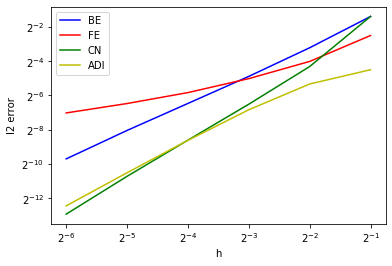
\includegraphics[width=1\textwidth]{immagini/validation_log-error}\caption{\label{fig:Err_par}Plot of the error \ref{eq:err_l2} in logarithmic
scale.}
\end{figure}

\begin{figure}[H]
\noindent \centering{}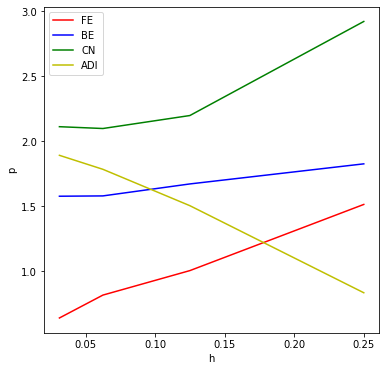
\includegraphics[width=1\textwidth]{immagini/validation_r}\caption{\label{fig:Conv_rate_par}Plot of the convergence rates \ref{eq:conv_rate}
of Forward Euler (FE), Backward Euler (BE), Crank-Nicolson (CN), Alternating
direction implicit method (ADI).}
\end{figure}
As expected, Forward Euler and Backward Euler have a lower convergence
rate than ADI and Crank-Nicolson. In this particular case, BE has
$p\approx1.5$ that is higher than what we expect. This is due, probably,
to a particularly simple manufactured solution. While both CN and
ADI reach $p=2$ with about $h\approx0.05$.

\section{The hyperbolic dynamics\label{sec:Hyperbolic-dynamic}}

The equation $\ref{eq:vick}$ has a drawback (the same of the Fourier
equation): \textit{the speed of information propagation is faster
than the speed of light in vacuum}. In 2010, Amadori, Boccabella and
Natalini \cite{amadori_one_2010} to overcome this problem proposed
a new 1-D spatial version of the replicator equation with finite speed
of propagation (similarly to Cattaneo works for the Fourier equation):
\begin{equation}
\begin{cases}
\frac{\partial n_{\ell}}{\partial t} & =-\frac{\partial\omega_{\ell}}{\partial x}+n_{\ell}\left[\frac{\mathbf{e_{\ell}}^{T}A\,\mathbf{n}}{N}-\frac{\mathbf{n}^{T}A\,\mathbf{n}}{N^{2}}\right]\\
\tau\frac{\partial\omega_{\ell}}{\partial t} & =-\lambda_{\ell}^{2}\frac{\partial n_{i}}{\partial x}-\omega_{\ell}
\end{cases}\qquad\ell=1,2.\label{eq:natal}
\end{equation}
Here $\mathbf{\omega_{\ell}}$ is the flux, $\tau$ is the relaxation
time and $\lambda_{\ell}$ is related to the dispersal rate. We extend
\ref{eq:natal} to two dimensions:
\begin{equation}
\begin{cases}
\frac{\partial n_{\ell}}{\partial t} & =-\left(\frac{\partial\varphi_{\ell}}{\partial x}+\frac{\partial\psi_{\ell}}{\partial y}\right)+n_{\ell}\left[\frac{\mathbf{e_{\ell}}^{T}A\,\mathbf{n}}{N}-\frac{\mathbf{n}^{T}A\,\mathbf{n}}{N^{2}}\right]\\
\tau\frac{\partial\varphi_{\ell}}{\partial t} & =-\lambda_{\ell}^{2}\frac{\partial n_{\ell}}{\partial x}-\varphi_{\ell}\\
\tau\frac{\partial\psi_{\ell}}{\partial t} & =-\lambda_{\ell}^{2}\frac{\partial n_{\ell}}{\partial y}-\psi_{\ell}
\end{cases}\qquad\ell=1,2\label{eq:2d_nat}
\end{equation}
 here $\varphi_{\ell}$ is the flux along $x$ and $\psi_{\ell}$
the one along $y$. In more dimensions and in a more compact form
the equation is:
\[
\begin{cases}
\frac{\partial n_{\ell}}{\partial t} & =-\bm{\nabla}\cdot\bm{\omega}_{\ell}+n_{\ell}\left[\frac{\mathbf{e_{\ell}}^{T}A\,\mathbf{n}}{N}-\frac{\mathbf{n}^{T}A\,\mathbf{n}}{N^{2}}\right]\\
\tau\frac{\partial\bm{\omega}_{\ell}}{\partial t} & =-\lambda_{\ell}^{2}\nabla n_{\ell}-\bm{\omega}_{\ell}
\end{cases}\qquad\ell=1,2
\]
whe\textcolor{black}{re $\bm{\omega}_{\ell}=\left(\begin{array}{c}
\varphi_{\ell}\\
\psi_{\ell}
\end{array}\right)$ is the flux vector of the population $\ell$.}

\textcolor{black}{We can study the evolution of the total number density.
Using the source term, i.e. \ref{eq:source}, we have from the first
pair of equations:
\begin{align*}
\frac{\partial N}{\partial t} & =\frac{\partial n_{1}}{\partial t}+\frac{\partial n_{2}}{\partial t}=\\
 & =-\left(\frac{\partial\varphi_{1}}{\partial x}+\frac{\partial\psi_{1}}{\partial y}\right)-\left(\frac{\partial\varphi_{2}}{\partial x}+\frac{\partial\psi_{2}}{\partial y}\right)-g\left(\mathbf{n}\right)+g\left(\mathbf{n}\right)\\
 & =-\frac{\partial}{\partial x}\left(\varphi_{1}+\varphi_{2}\right)-\frac{\partial}{\partial y}\left(\psi_{1}+\psi_{2}\right)=-\bm{\nabla}\cdot\left(\bm{\omega}_{1}+\bm{\omega}_{2}\right)
\end{align*}
The total population living in $\left(0,L_{x}\right)\times\left(0,L_{y}\right)$
is given by:
\begin{equation}
\tilde{N}\left(t\right)\coloneqq\intop_{0}^{L_{y}}\intop_{0}^{L_{x}}N\left(\mathbf{x},t\right)dx\,dy\label{eq:N_tot}
\end{equation}
 and its variation in time is:
\begin{align}
\frac{d\tilde{N}\left(t\right)}{dt} & =\intop_{0}^{L_{y}}\intop_{0}^{L_{x}}\frac{\partial N}{\partial t}dx\,dy=-\intop_{0}^{L_{y}}\intop_{0}^{L_{x}}-\bm{\nabla}\cdot\left(\bm{\omega}_{1}+\bm{\omega}_{2}\right)dx\,dy.\label{eq:N_nat}
\end{align}
This is essentially the same of \ref{eq:N_vick}, i.e. $N$ can only
change by the flux of player across the boundary of the considered
region.}

We will study the dynamics \ref{eq:2d_nat} on a two dimensional plane
$\left[0,L_{x}\right]\times\left[0,L_{y}\right]$ in a time interval
$\left[0,T\right]$ with the following initial conditions:
\begin{align*}
\begin{cases}
n_{1}\left(x,y,0\right) & =n_{1}^{0}\left(x,y\right)\\
\varphi_{1}\left(x,y,0\right) & =0\\
\psi_{1}\left(x,y,0\right) & =0\\
n_{2}\left(x,y,0\right) & =n_{2}^{0}\left(x,y\right)\\
\varphi_{2}\left(x,y,0\right) & =0\\
\psi_{2}\left(x,y,0\right) & =0
\end{cases}
\end{align*}
we choose zero value initial flux, but we consider three forms of
$n_{1}^{0}\left(x,y\right)$ and $n_{2}^{0}\left(x,y\right)$:
\begin{enumerate}
\item a random value between $0$ to $1$, i.e. for $\ell=1,2$:
\[
\forall x,y\quad n_{\ell}^{0}\left(x,y\right)=random\left[0,1\right];
\]
\item a single defector in a sea of cooperators, i.e. for the cooperators:
\[
n_{1}^{0}\left(x,y\right)=\begin{cases}
1 & if\ x\neq\frac{L_{x}}{2}\ or\ y\neq\frac{L_{y}}{2}\\
0 & otherwise
\end{cases}
\]
 and for the defectors:
\[
n_{2}^{0}\left(x,y\right)=\begin{cases}
1 & if\ x=\frac{L_{x}}{2}\ and\ y=\frac{L_{y}}{2}\\
0 & otherwise
\end{cases};
\]
\item a delta-type of defectors, rather the defectors are distributed along
a segment surrounded by cooperators, i.e.:
\begin{align*}
n_{1}^{0}\left(x,y\right) & =\begin{cases}
1 & if\ x\neq\frac{L_{x}}{2}\\
0 & otherwise
\end{cases}\\
n_{2}^{0}\left(x,y\right) & =\begin{cases}
1 & if\ x=\frac{L_{x}}{2}\\
0 & otherwise
\end{cases}
\end{align*}
\end{enumerate}
As done in section \ref{sec:Parabolic-dynamic}, the boundary conditions
are always zero, i.e. for $\ell=1,2$:
\begin{align*}
n_{\ell}\left(0,0,t\right) & =n_{\ell}\left(0,L_{y},t\right)=n_{\ell}\left(L_{x},0,t\right)=n_{\ell}\left(L_{x},L_{y},t\right)=0\quad\forall t\in\left[0,T\right]\\
\varphi_{\ell}\left(0,0,t\right) & =\varphi_{\ell}\left(0,L_{y},t\right)=\varphi_{\ell}\left(L_{x},0,t\right)=\varphi_{\ell}\left(L_{x},L_{y},t\right)=0\quad\forall t\in\left[0,T\right]\\
\psi_{\ell}\left(0,0,t\right) & =\psi_{\ell}\left(0,L_{y},t\right)=\psi_{\ell}\left(L_{x},0,t\right)=\psi_{\ell}\left(L_{x},L_{y},t\right)=0\quad\forall t\in\left[0,T\right]
\end{align*}

Moreover, we can see that equation \ref{eq:2d_nat} is a hyperbolic
PDE, so we use and compare two finite-difference methods, namely the
Lax method and the Lax-Wendroff method (for more details \cite{ames_numerical_1992,press_numerical_2007,pang_introduction_2006,thomas1995numerical,thomas1999numerical}).

Moreover, we can see that equation \ref{eq:2d_nat} is a hyperbolic
PDE. We use two finite difference algorithms:
\begin{itemize}
\item Lax;
\item Lax-Wendroff.
\end{itemize}

\subsection{Lax}

Lax method \cite{press_numerical_2007} is one of the most simple
finite difference explicit algorithm. Preserving the notation adopted
above, the first equation of the system can be written:

\begin{align*}
\frac{1}{\Delta t}\left\{ \left(n_{\ell}\right)_{i,j}^{k+1}-\frac{1}{4}\left[\left(n_{\ell}\right)_{i+1,j}^{k}\right.\right.\\
\left.\left.+\left(n_{\ell}\right)_{i-1,j}^{k}+\left(n_{\ell}\right)_{i,j+1}^{k}+\left(n_{\ell}\right)_{i,j-1}^{k}\right]\right\}  & =-\frac{\left(\varphi_{\ell}\right)_{i+1,j}^{k}-\left(\varphi_{\ell}\right)_{i-1,j}^{k}}{\Delta x}\\
 & -\frac{\left(\psi_{\ell}\right)_{i,j+1}^{k}-\left(\psi_{\ell}\right)_{i,j-1}^{k}}{\Delta y}\\
 & +\left(-1\right)^{\ell}\frac{\left(n_{1}\right)_{i.j}^{k}\left(n_{2}\right)_{i,j}^{k}}{\left(\left(n_{1}\right)_{i.j}^{k}+\left(n_{2}\right)_{i.j}^{k}\right)^{2}}\left(b-1\right)\left(n_{1}\right)_{i.j}^{k}
\end{align*}
 the second equation becomes:
\begin{align*}
\tau\frac{\left(\varphi_{\ell}\right)_{i,j}^{k+1}-\frac{1}{2}\left[\left(\varphi_{\ell}\right)_{i+1,j}^{k}+\left(\varphi_{\ell}\right)_{i-1,j}^{k}\right]}{\Delta t}= & -\left(\varphi_{\ell}\right)_{i,j}^{k}\\
 & -\lambda_{\ell}^{2}\frac{\left(n_{\ell}\right)_{i+1,j}^{k}-\left(n_{\ell}\right)_{i-1,j}^{k}}{\Delta x}
\end{align*}
 and for the third equation we have:
\begin{align*}
\tau\frac{\left(\psi_{\ell}\right)_{i,j}^{k+1}-\frac{1}{2}\left[+\left(\psi_{\ell}\right)_{i,j+1}^{k}+\left(\psi_{\ell}\right)_{i,j-1}^{k}\right]}{\Delta t} & =-\left(\psi_{\ell}\right)_{i,j}^{k}\\
 & -\lambda_{\ell}^{2}\frac{\left(n_{\ell}\right)_{i,j+1}^{k}-\left(n_{\ell}\right)_{i,j-1}^{k}}{\Delta y}.
\end{align*}
And so, we have the updating formulae:
\begin{align}
\left(n_{\ell}\right)_{i,j}^{k+1}= & \frac{1}{4}\left[\left(n_{\ell}\right)_{i+1,j}^{k}+\left(n_{\ell}\right)_{i-1,j}^{k}+\left(n_{\ell}\right)_{i,j+1}^{k}+\left(n_{\ell}\right)_{i,j-1}^{k}\right]\nonumber \\
 & -\Delta t\frac{\left(\varphi_{\ell}\right)_{i+1,j}^{k}-\left(\varphi_{\ell}\right)_{i-1,j}^{k}}{\Delta x}\nonumber \\
 & -\Delta t\frac{\left(\psi_{\ell}\right)_{i,j+1}^{k}-\left(\psi_{\ell}\right)_{i,j-1}^{k}}{\Delta y}\nonumber \\
 & +\Delta t\left(-1\right)^{\ell}\frac{\left(n_{1}\right)_{i.j}^{k}\left(n_{2}\right)_{i,j}^{k}}{\left(\left(n_{1}\right)_{i.j}^{k}+\left(n_{2}\right)_{i.j}^{k}\right)^{2}}\left(b-1\right)\left(n_{1}\right)_{i.j}^{k}\nonumber \\
\left(\varphi_{\ell}\right)_{i,j}^{k+1}= & \frac{1}{2}\left[\left(\varphi_{\ell}\right)_{i+1,j}^{k}+\left(\omega_{\ell}\right)_{i-1,j}^{k}\right]\nonumber \\
 & -\frac{\lambda_{\ell}^{2}}{\tau}\frac{\left(n_{\ell}\right)_{i+1,j}^{k}-\left(n_{\ell}\right)_{i-1,j}^{k}}{\Delta x}\nonumber \\
 & -\frac{\left(\varphi_{\ell}\right)_{i,j}^{k}}{\tau}.\nonumber \\
\left(\psi_{\ell}\right)_{i,j}^{k+1}= & \frac{1}{2}\left[\left(\psi_{\ell}\right)_{i,j+1}^{k}+\left(\psi_{\ell}\right)_{i,j-1}^{k}\right]\nonumber \\
 & -\frac{\lambda_{\ell}^{2}}{\tau}\frac{\left(n_{\ell}\right)_{i,j+1}^{k}-\left(n_{\ell}\right)_{i,j-1}^{k}}{\Delta y}\nonumber \\
 & -\frac{\left(\psi_{\ell}\right)_{i,j}^{k}}{\tau}.\label{eq:lax}
\end{align}


\subsection{Lax-Wendroff }

In 1960, Lax and Wendroff developed in their paper \cite{lax_systems_1960}
an explicit numerical scheme for hyperbolic PDE, based on the central
differences in space and second order Taylor expansion in time. In
two spatial dimension:
\begin{align*}
\left(n_{\ell}\right)_{i,j}^{k+1}= & \left(n_{\ell}\right)_{i,j}^{k}\\
 & -\frac{1}{2}\frac{\Delta t}{\Delta x}\left(\left(\varphi_{\ell}\right)_{i+1,j}^{k}-\left(\varphi_{\ell}\right)_{i-1,j}^{k}\right)\\
 & -\frac{1}{2}\frac{\Delta t}{\Delta y}\left(\left(\psi_{\ell}\right)_{i,j+1}^{k}-\left(\psi_{\ell}\right)_{i,j-1}^{k}\right)\\
 & +\frac{\Delta t^{2}}{2\Delta x^{2}}\left(\left(\varphi_{\ell}\right)_{i+1,j}^{k}-2\left(\varphi_{\ell}\right)_{i,j}^{k}+\left(\varphi_{\ell}\right)_{i-1,j}^{k}\right)\\
 & +\frac{\Delta t^{2}}{2\Delta y^{2}}\left(\left(\psi_{\ell}\right)_{i,j+1}^{k}-2\left(\psi_{\ell}\right)_{i,j}^{k}+\left(\psi_{\ell}\right)_{i,j-1}^{k}\right)\\
 & +\Delta t\left(-1\right)^{\ell}\frac{\left(n_{1}\right)_{i.j}^{k}\left(n_{2}\right)_{i,j}^{k}}{\left(\left(n_{1}\right)_{i.j}^{k}+\left(n_{2}\right)_{i.j}^{k}\right)^{2}}\left(b-1\right)\left(n_{1}\right)_{i.j}^{k}\\
\left(\varphi_{\ell}\right)_{i,j}^{k+1}= & \left(\varphi_{\ell}\right)_{i,j}^{k}\\
 & -\frac{\lambda_{\ell}^{2}}{2\tau}\frac{\Delta t}{\Delta x}\left(\left(n_{\ell}\right)_{i+1,j}^{k}-\left(n_{\ell}\right)_{i-1,j}^{k}\right)\\
 & +\frac{\lambda_{\ell}^{4}}{2\tau^{2}}\frac{\Delta t^{2}}{\Delta x^{2}}\left(\left(n_{\ell}\right)_{i+1,j}^{k}-2\left(n_{\ell}\right)_{i,j}^{k}+\left(n_{\ell}\right)_{i-1,j}^{k}\right)\\
 & -\frac{\left(\varphi_{\ell}\right)_{i,j}^{k}}{\tau}\\
\left(\psi_{\ell}\right)_{i,j}^{k+1}= & \left(\psi_{\ell}\right)_{i,j}^{k}\\
 & -\frac{\lambda_{\ell}^{2}}{2\tau}\frac{\Delta t}{\Delta y}\left(\left(n_{\ell}\right)_{i,j+1}^{k}-\left(n_{\ell}\right)_{i,j-1}^{k}\right)\\
 & +\frac{\lambda_{\ell}^{4}}{2\tau^{2}}\frac{\Delta t^{2}}{\Delta y^{2}}\left(\left(n_{\ell}\right)_{i,j+1}^{k}-2\left(n_{\ell}\right)_{i,j}^{k}+\left(n_{\ell}\right)_{i,j-1}^{k}\right)\\
 & -\frac{\left(\psi_{\ell}\right)_{i,j}^{k}}{\tau}
\end{align*}


\subsection{A drawback}

Finite difference methods have a big limit, well described by Godunov's
theorem \cite{Godunov54,Godunov59}:
\begin{thm}
Assume a continuum problem described by a PDE is to be computed using
a numerical scheme based upon a uniform computational grid and a one-step,
constant step-size, $M$ grid points integration algorithm, either
implicit or explicit. Writing $x_{j}=j\Delta x$ and $t_{n}=n\Delta t$,
such a scheme can be described by:
\[
\varphi_{j}^{n+1}=\sum\limits _{m}^{M}{\gamma_{m}\varphi_{j+m}^{n}}
\]
Then the above scheme is monotonicity preserving, i.e.:
\[
if\quad\varphi_{j+1}^{n}\geq\varphi_{j}^{n}\quad\forall j\Rightarrow\varphi_{j+1}^{n+1}\geq\varphi_{j}^{n+1}\quad\forall j
\]
 if and only if: 

\[
\gamma_{m}\ge0,\quad\forall m
\]
\end{thm}

In other words, it establishes that a monotone behaviour of a numerical
solution cannot be assured for linear finite-difference methods with
more than first-order accuracy (for more details \cite{tryggvason_lecture_2017,thirumgam_numerical_2012}).
This problem is clear in fig \ref{fig:oscill_example}, where we compared
the Lax and Lax-Wendroff methods for our one-dimensional problem.

\begin{figure}
\subfloat[]{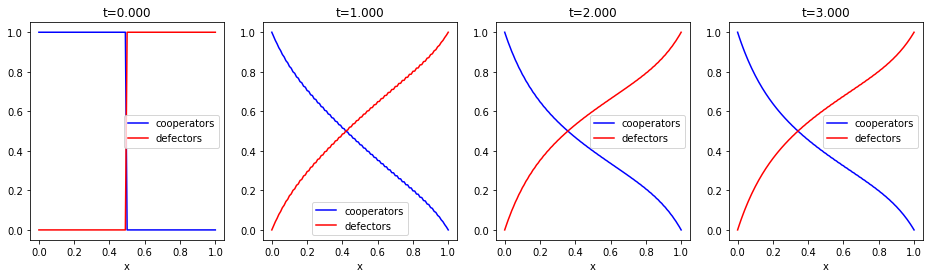
\includegraphics[width=1\textwidth]{immagini/lax_example}

}

\subfloat[]{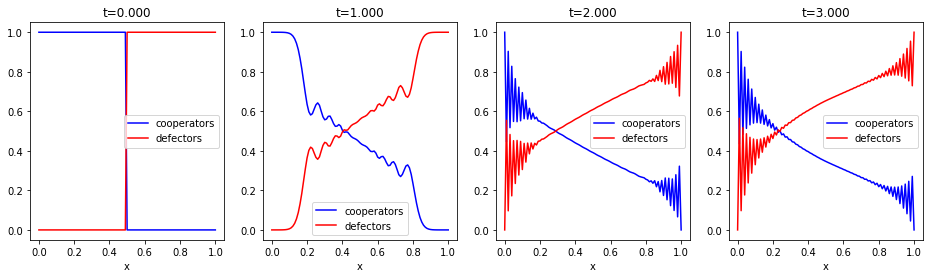
\includegraphics[width=1\textwidth]{immagini/l-w_example}

}

\caption{\label{fig:oscill_example}Numerical solution of $n_{1}$ and $n_{2}$
of \ref{eq:natal} with $T=3$ and $L_{x}=1.0$, setting $\lambda=0.3$,
$\tau=0.8$ and $b=1.85$, with Lax method (A) and Lax-Wendroff one
(B). The boundary condition are $n_{1}(0,t)=1$, $n_{1}(L_{x},t)=0$,
$n_{2}(0,t)=0$ and $n_{2}(L_{x},t)=1$.}

\end{figure}

As expected, the solutions of the Lax-Wendroff are not monotonic.
One way to overcome this limit is to use \textit{artificial viscosity}
\cite{vonneumann_method_1950,Biringen2011}. In practice, a term of
artificial dissipation is added to smooth the numerical solutions.
Considering \ref{eq:natal}, this term is written as:
\begin{align*}
q_{n_{\ell}} & =\mu_{n}\left(\left(n_{\ell}\right)_{i+1}^{k}-2\left(n_{\ell}\right)_{i}^{k}+\left(n_{\ell}\right)_{i-1}^{k}\right)\\
q_{\varphi_{\ell}} & =\mu_{\varphi}\left(\left(\varphi_{\ell}\right)_{i+1}^{k}-2\left(\varphi_{\ell}\right)_{i}^{k}+\left(\varphi_{\ell}\right)_{i-1}^{k}\right)\\
q_{\psi_{\ell}} & =\mu_{\psi}\left(\left(\psi_{\ell}\right)_{i+1}^{k}-2\left(\psi_{\ell}\right)_{i}^{k}+\left(\psi_{\ell}\right)_{i-1}^{k}\right)
\end{align*}

where $\mu_{n}$, $\mu_{\varphi}$ and $\mu_{\psi}$ are two constants
in $\left[0,1\right]$. How the artificial viscosity modifies the
results are quite controversial, but it has been used often. We can
see the reason why in fig \ref{fig:art_visc_example}.

\begin{figure}
\subfloat[]{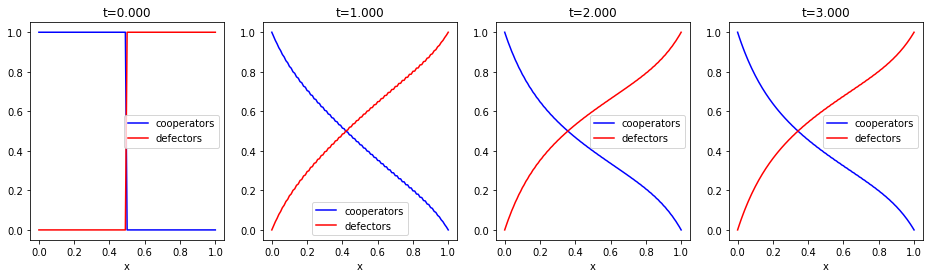
\includegraphics[width=1\textwidth]{immagini/lax_example}

}

\subfloat[]{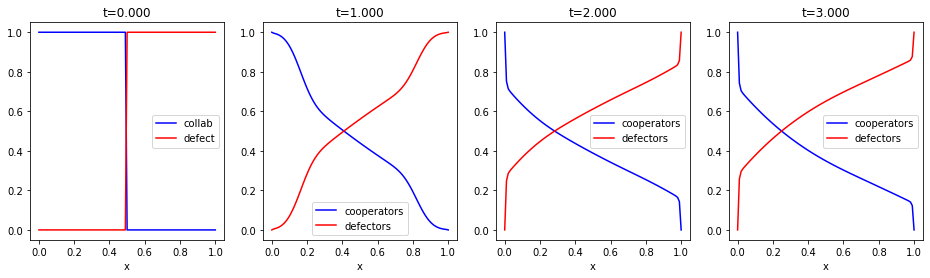
\includegraphics[width=1\textwidth]{immagini/l-w-av_example}

}

\caption{\label{fig:art_visc_example}Numerical solution of $n_{1}$ and $n_{2}$
of \ref{eq:natal} with $T=3$ and $L_{x}=1.0$, setting $\lambda=0.3$,
$\tau=0.8$ and $b=1.85$, with Lax method (A) and Lax-Wendroff one
with artificial viscosity with $\mu_{n}=\mu_{\omega}=0.05$ (B). The
boundary condition are $n_{1}(0,t)=1$, $n_{1}(L_{x},t)=0$, $n_{2}(0,t)=0$
and $n_{2}(L_{x},t)=1$.}
\end{figure}

In our work, we choose $\mu_{n}$, $\mu_{\varphi}$ and $\mu_{\psi}$
empirically.

\subsection{Verification}

Now, we can verify the code, as seen above. The chosen \textit{manufactured
solutions} for the hyperbolic model are:
\begin{align*}
n_{1ex}\left(x,y,t\right) & =5e^{\text{\textminus}2\frac{t}{\tau}}\left(x-L_{x}\right)\left(y-L_{y}\right),\\
\varphi_{1ex}\left(x,y,t\right) & =1,\\
\psi_{1ex}\left(x,y,t\right) & =1,\\
n_{2ex}\left(x,y,t\right) & =e^{\text{\textminus}2\frac{t}{\tau}}\left(x-L_{x}\right)\left(y-L_{y}\right),\\
\varphi_{2ex}\left(x,y,t\right) & =1,\\
\psi_{2ex}\left(x,y,t\right) & =1.
\end{align*}

And so, inserting them in \ref{eq:2d_nat}, the source terms are (computed
with \textit{sympy}):

\begin{align*}
f_{n_{1}}= & 0.069\bar{4}\left(x-L_{x}\right)\left(y-L_{y}\right)e^{\text{\textminus}2\frac{t}{\tau}}-\frac{2}{\tau}(5x-5L_{x})(y-L_{y})e^{\text{\textminus}2\frac{t}{\tau}}\\
f_{\varphi_{1}}= & \lambda^{2}e^{\text{\textminus}2\frac{t}{\tau}}(5y-5L_{y})+1\\
f_{\psi_{1}}= & \lambda^{2}e^{\text{\textminus}2\frac{t}{\tau}}(5x-5L_{x})+1\\
f_{n_{2}}= & -0.069\bar{4}\left(x-L_{x}\right)\left(y-L_{y}\right)e^{\text{\textminus}2\frac{t}{\tau}}-\frac{2}{\tau}(x-L_{x})(y-L_{y})e^{\text{\textminus}2\frac{t}{\tau}}\\
f_{\varphi_{2}}= & \lambda^{2}e^{\text{\textminus}2\frac{t}{\tau}}(y-L_{y})+1\\
f_{\psi_{2}}= & \lambda^{2}e^{\text{\textminus}2\frac{t}{\tau}}(x-L_{x})+1
\end{align*}

Then, we can compute the $\ell^{2}$ error:
\begin{align}
E_{n_{1}} & =\sqrt{\Delta x\:\Delta y\:\sum_{j=0}^{N_{y}}\:\sum_{i=0}^{N_{x}}\left(n_{1ex}\left(i\cdot dx,\,j\cdot dy,\,T\right)-\left(n_{1}\right)_{i,j}^{N_{t}}\right)},\label{eq:err_l2_hyp}\\
E_{\varphi_{1}} & =\sqrt{\Delta x\:\Delta y\:\sum_{j=0}^{N_{y}}\:\sum_{i=0}^{N_{x}}\left(\varphi_{1ex}\left(i\cdot dx,\,j\cdot dy,\,T\right)-\left(\varphi_{1}\right)_{i,j}^{N_{t}}\right)},\nonumber \\
E_{\psi_{1}} & =\sqrt{\Delta x\:\Delta y\:\sum_{j=0}^{N_{y}}\:\sum_{i=0}^{N_{x}}\left(\psi_{1ex}\left(i\cdot dx,\,j\cdot dy,\,T\right)-\left(\psi_{1}\right)_{i,j}^{N_{t}}\right)},\nonumber \\
E_{n_{2}} & =\sqrt{\Delta x\:\Delta y\:\sum_{j=0}^{N_{y}}\:\sum_{i=0}^{N_{x}}\left(n_{2ex}\left(i\cdot dx,\,j\cdot dy,\,T\right)-\left(n_{2}\right)_{i,j}^{N_{t}}\right)},\nonumber \\
E_{\varphi_{2}} & =\sqrt{\Delta x\:\Delta y\:\sum_{j=0}^{N_{y}}\:\sum_{i=0}^{N_{x}}\left(\varphi_{2ex}\left(i\cdot dx,\,j\cdot dy,\,T\right)-\left(\varphi_{2}\right)_{i,j}^{N_{t}}\right)},\nonumber \\
E_{\psi_{2}} & =\sqrt{\Delta x\:\Delta y\:\sum_{j=0}^{N_{y}}\:\sum_{i=0}^{N_{x}}\left(\psi_{2ex}\left(i\cdot dx,\,j\cdot dy,\,T\right)-\left(\psi_{2}\right)_{i,j}^{N_{t}}\right)}\nonumber 
\end{align}
 Now, we can plot the error (fig \ref{fig:Err_hyp}) and the convergence
rates (fig \ref{fig:Conv_rate_hyp}).

\begin{figure}[H]
\noindent \centering{}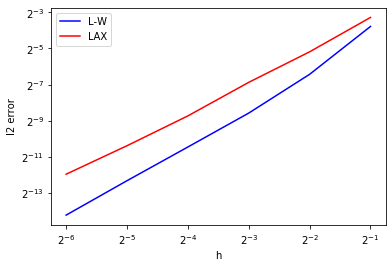
\includegraphics[width=1\textwidth]{immagini/validation_log-error_hyp}\caption{\foreignlanguage{english}{\label{fig:Err_hyp}Plot of the error \ref{eq:err_l2_hyp} in logarithmic
scale.}}
\end{figure}

\begin{figure}[H]
\noindent \centering{}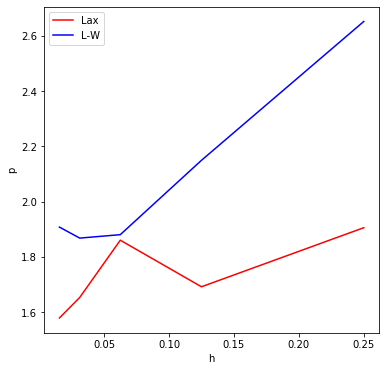
\includegraphics[width=1\textwidth]{immagini/validation_r_hyp}\caption{\foreignlanguage{english}{\label{fig:Conv_rate_hyp}Plot of the convergence rates \ref{eq:conv_rate}
of Lax method and Lax-Wendroff method (L-W).}}
\end{figure}

We can observe that (after some fluctuations), the Lax-Wendroff method
converges to $p=2$, while the Lax one converges to smaller $p$.

\section{The simulations\label{sec:The-simulations}}

We solve the parabolic model \ref{eq:vick} and the hyperbolic model
\ref{eq:2d_nat} with the Crank-Nicolson for the former and the Lax-Wendroff
for the latter. As anticipated, we choose three different initial
conditions:
\begin{enumerate}
\item random spatial distribution of cooperators and defectors;
\item a single defector in a sea of cooperators;
\item a delta-type of defectors surrounded by cooperators.
\end{enumerate}

\subsection{Random initial condition}

In this simulation we assume an initial random distribution of cooperators
and defectors (fig \ref{fig:rand}). 

\begin{figure}
\subfloat[]{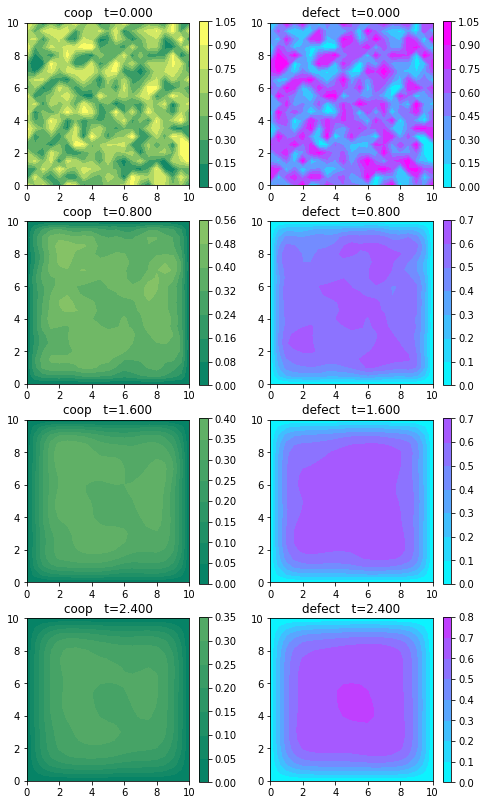
\includegraphics[width=0.5\textwidth]{immagini/CN-rand}

}\subfloat[]{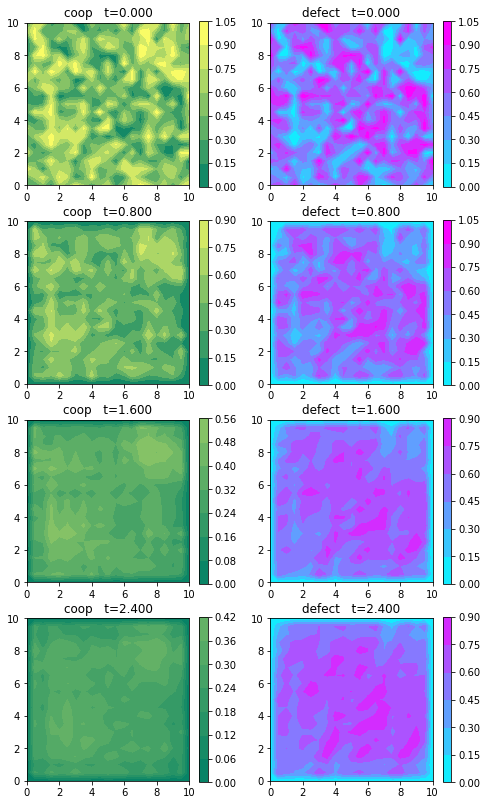
\includegraphics[width=0.5\textwidth]{immagini/l-w-rand}

}\caption{\label{fig:rand}Numerical solution of $n_{1}$ and $n_{2}$ in $T=2.4$
and $L_{x}=L_{y}=10$ of parabolic model \ref{eq:vick} using Crank-Nicolson
with $D=0.25$ (A) and hyperbolic model \ref{eq:2d_nat} using Lax-Wendroff
with artificial viscosity with $\mu_{n}=\mu_{\varphi}=\mu_{\psi}=0.001$,
$\lambda=0.5$ and $\tau=0.9$ (B). For both the methods we set $N_{x}=N_{y}=20$,
$dt=0.01$ and $b=1.85$.}
\end{figure}


\subsection{One defector in a sea of cooperators}

Second, we study the two equations setting at the starting time the
defectors in a single central point (fig \ref{fig:onedef}). 

\begin{figure}
\subfloat[]{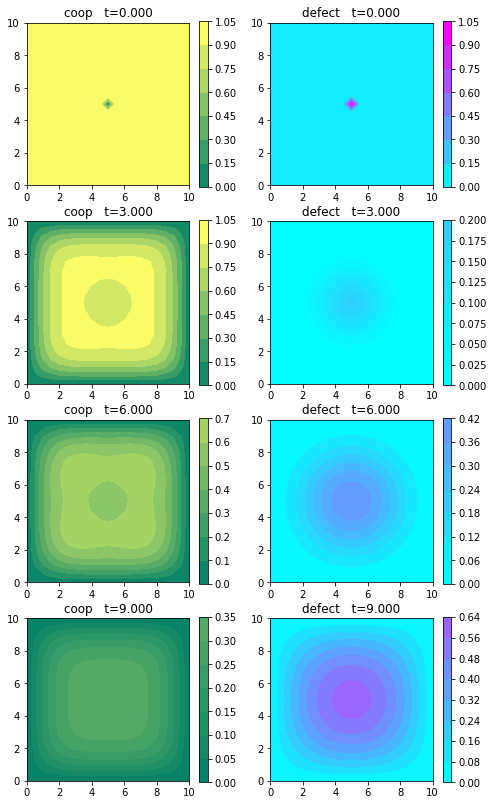
\includegraphics[width=0.5\textwidth]{immagini/CN-onedef}

}\subfloat[]{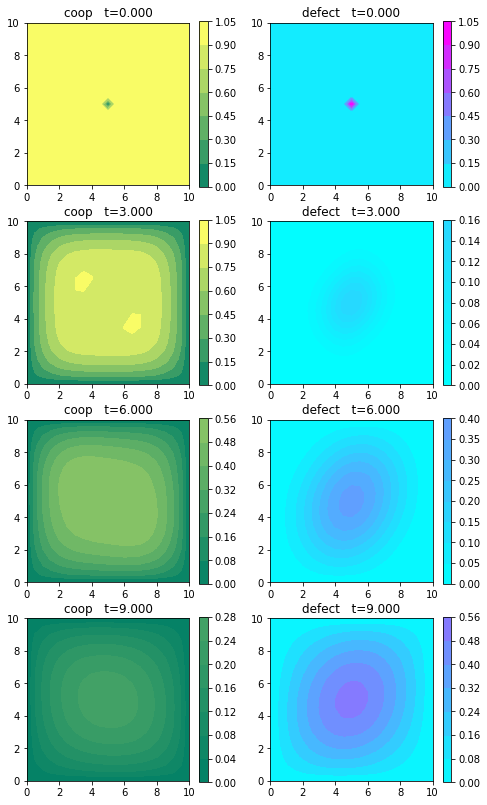
\includegraphics[width=0.5\textwidth]{immagini/l-w-onedef}

}

\caption{\label{fig:onedef}Numerical solution of $n_{1}$ and $n_{2}$ in
$T=9$ and $L_{x}=L_{y}=10$ of parabolic model \ref{eq:vick} using
Crank-Nicolson with $D=0.25$ (A) and hyperbolic model \ref{eq:2d_nat}
using Lax-Wendroff with artificial viscosity with $\mu_{n}=\mu_{\varphi}=\mu_{\psi}=0.001$,
$\lambda=0.5$ and $\tau=0.9$ (B). For both the methods we set $N_{x}=N_{y}=20$,
$dt=0.01$ and $b=1.85$.}
\end{figure}


\subsection{Delta initial condition}

Finally, we analyse the two models, arranging the defectors in delta-type
function in the space surrounded by the cooperators, at the initial
time (fig \ref{fig:delta}). 

\begin{figure}
\subfloat[]{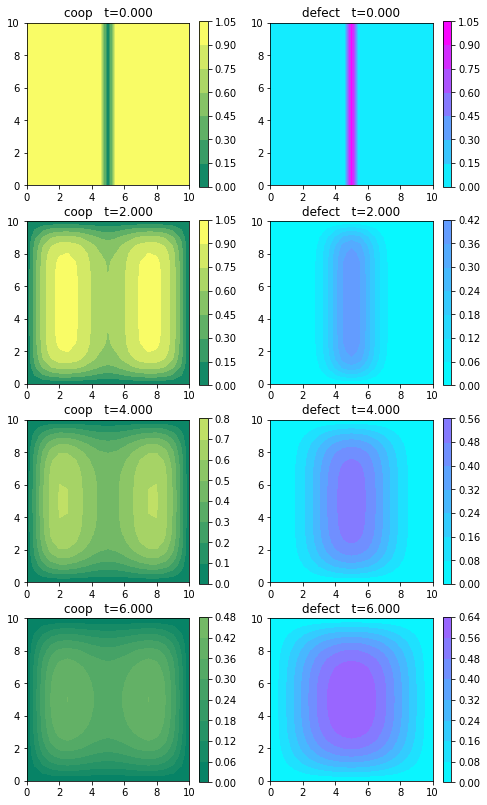
\includegraphics[width=0.5\textwidth]{immagini/CN-delta}

}\subfloat[]{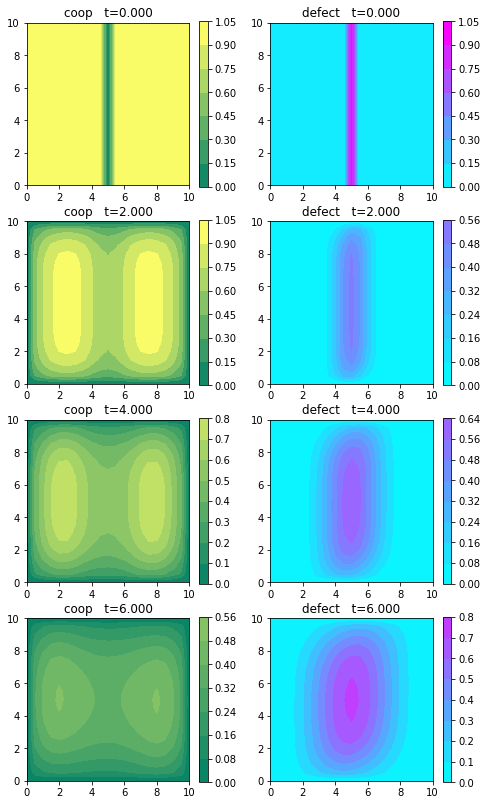
\includegraphics[width=0.5\textwidth]{immagini/l-w-delta}

}

\caption{\label{fig:delta}Numerical solution of $n_{1}$ and $n_{2}$ in $T=6$
and $L_{x}=L_{y}=10$ of parabolic model \ref{eq:vick} using Crank-Nicolson
with $D=0.25$ (A) and hyperbolic model \ref{eq:2d_nat} using Lax-Wendroff
with artificial viscosity with $\mu_{n}=\mu_{\varphi}=\mu_{\psi}=0.005$,
$\lambda=0.5$ and $\tau=0.9$ (B). For both the methods we set $N_{x}=N_{y}=20$,
$dt=0.01$ and $b=1.85$.}
\end{figure}


\subsection{Phase diagram and conclusion}

In brief, we can see that the evolution in the parabolic and hyperbolic
models is quite similar, and the defectors invade the whole of the
space and the population of cooperators becomes extinct. The hyperbolic
model needs more time to diffuse the population, but this is what
we expect because a limited speed is explicitly requested.

Now we want to try to understand the evolution as $b$ varies. Instead
of plotting the evolution of the populations in the space for each
value, we use the phase diagrams of the probability of a strategy
varying $b$. To obtain the probability of one of the strategies,
we must compute:
\[
p_{\ell}=\frac{\frac{1}{L_{x}L_{y}}\int_{0}^{L_{X}}\int_{0}^{L_{y}}n_{i}(x,y,t)dxdy}{\frac{1}{L_{x}L_{y}}\int_{0}^{L_{X}}\int_{0}^{L_{y}}\sum_{j}n_{j}(x,y,t)dxdy}\qquad t\rightarrow+\infty
\]

\begin{figure}
\subfloat[]{

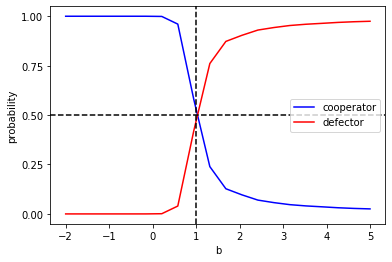
\includegraphics[width=0.5\textwidth]{immagini/CN_phase}

}\subfloat[]{

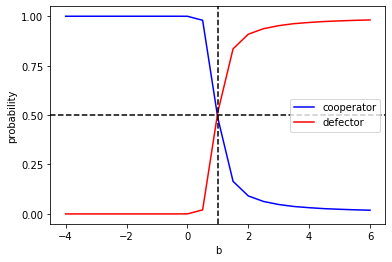
\includegraphics[width=0.5\textwidth]{immagini/l-w_phase}

}\caption{Phase diagrams of the parabolic model (A) and of the hyperbolic model
(B).}

\end{figure}

Not so surprisingly, we observe a phase transition when $b=1$. Recalling
the payoff matrix:
\[
A=\left(\begin{array}{cc}
R & S\\
T & P
\end{array}\right)=\left(\begin{array}{cc}
1 & 0\\
b & 0
\end{array}\right)
\]
 we have a phase transition when the payoff of the defection (i.e.
the temptation $T$) becomes higher than the one for the cooperation
(i.e. the reward $R$). 
